%卒論概要テンプレート ver. 4.0

\documentclass[uplatex,twocolumn,dvipdfmx]{jsarticle}
\usepackage[top=22mm,bottom=22mm,left=22mm,right=22mm]{geometry}
\setlength{\columnsep}{11mm}
\usepackage[T1]{fontenc}
\usepackage{txfonts}
\usepackage[expert,deluxe]{otf}
\usepackage[dvipdfmx,hiresbb]{graphicx}
\usepackage[dvipdfmx]{hyperref}
\usepackage{pxjahyper}
\usepackage{secdot}





%タイトルと学生番号,名前だけ編集すること
\title{\vspace{-5mm}\fontsize{14pt}{0pt}\selectfont Twitterのデマ拡散シュミレーション}
\author{\normalsize プロジェクトマネジメントコース 矢吹研究室 1442043 川崎貴雅}
\date{}
\pagestyle{empty}
\begin{document}
\fontsize{10.5pt}{\baselineskip}\selectfont
\maketitle



%以下が本文
\section{序論}\label{序論}

スマートフォンなどの普及と共にTwitterを始めとしたとしたマイクロブログが急激に普及している.Twitterはリアルタイムな情報を手軽に多くのユーザーへと伝播できるため社会に影響を与えている.例えば東日本大震災時のデマ情報が拡散された事や北朝鮮のミサイルを目撃したというデマが挙げられる.このようなツイートの拡散をシュミレーションで再現することができるのではないかと考えられる.

本研究ではTwitterを調査し,現実に近いデマ拡散のシュミレーションを再現することができるかを調査したい.
実際にデマ拡散シュミレーションを行うためには2つほど調べる事がある.1つは人は1日にどのくらいツイートするのか確認である.もう1つはツイートが拡散する様子をシュミレートする手法の確立をしておくことである.
また本研究は調べた2つをもとに現実的なシュミレーションを行えるかまでが目標の研究であるが,人は1日にどれくらいツイートするのかの確認とツイートの拡散する様子のシュミレーション手法の確立までしか出来ていないものである.



\section{目的}

本研究では現実のデマ拡散に近い状況をシュミレーションで再現できるか調査することである.

\section{手法}

デマの拡散シュミレートするために以下の手順で行う.
\begin{enumerate}
\item TwitterAPIを用いて1日のツイート数,フォロワー数などを取得し計算処理を行い1日の平均ツイート数を割り出す.
\item ツイートの拡散する様子をシュミレートする手法確立のため,ランダムグラフでグループを作成し実際にシュミレーションを動かしてみる\cite{netto}.
\item 現実に近いシュミレーションにするため上記2つを組み合わせたシュミレーションを行う.
\end{enumerate}
\begin{figure}[htb]
\centering
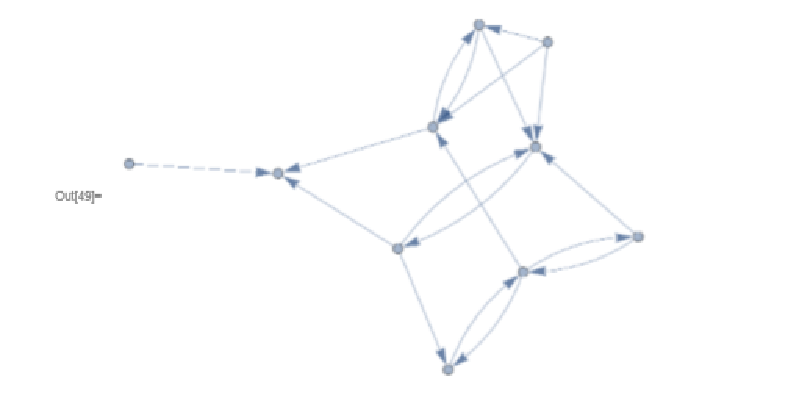
\includegraphics[width=55mm,clip]{rg.pdf}
\caption{10人が0.2の確率でつながっているランダムグラフ}\label{サンプル図}
\end{figure}
\section{結果}

50万人のデータから1日の平均ツイート数1.37542回であることが分かった,またグループ構築にランダムグラフを使ったツイートの拡散するシュミレートする手法の確立ができた.しかし平均ツイート数とツイート拡散のシュミレート手法を組み合わせた現実的なシュミレーションを行うことはできなかった.


\section{考察}

ランダムグラフでの現実的なシュミレーションを行う上で,集めた50万人のデータからフォロワー数の平均を割り出し,1日の平均ツイート数と合わせてシュミレーションをすることができたのではないのかと考えられる.

\section{結論}

本研究では1日あたりのツイート数の平均が分かったこととグループ構築にランダムグラフを使ったツイートの拡散するシュミレートする手法の確立ができた.現実に近いシュミレーションを行うことはできなかったが,Twitterのユーザーの平均フォロー人数がわかれば現実に近いシュミレーションができることが期待される.

\bibliographystyle{junsrt}
\bibliography{biblio}%「biblio.bib」というファイルが必要.

\end{document}
